\documentclass[a4paper, 11pt]{article}
\usepackage{geometry}
\usepackage{graphicx}
\usepackage{mathspec} % includes fontspec
\usepackage[natbibapa]{apacite}
\usepackage[font={small,sf}]{caption}

\geometry{a4paper,total={150mm,237mm},inner=30mm,top=30mm}
\defaultfontfeatures{Mapping=tex-text,Scale=MatchLowercase}
\setsansfont{Helvetica}
\setmonofont{Menlo}

\title{Simplicity and informativeness in semantic category systems \\ S3: Participant exclusion and attrition}
\author{Jon W. Carr, Kenny Smith, Jennifer Culbertson, Simon Kirby}
\date{}

\begin{document}
\maketitle

\section{Participant exclusion}

On every trial, the participant had to click one of four response buttons (or one of 64 response stimuli in the case of the Comprehension condition in Experiment~1). The mapping between labels/stimuli and buttons was randomized on every trial, such that the participant would have to look over the buttons to find they one they wanted. Therefore, we would expect to find that \textit{buttons} (but not necessarily labels/stimuli) are being clicked at random. If button clicks appear to be nonrandom, this would suggest that the participant is repeatedly clicking the same button without regard to the label (or stimulus). To check for this, we looked at the entropy of button clicks (see Fig.~\ref{fg_exclusion}). Random button clicking would result in entropy of $\log 4 = 2$~bits (Production) or $\log 64 = 6$~bits (Comprehension).

	\begin{figure}
	\begin{center}
	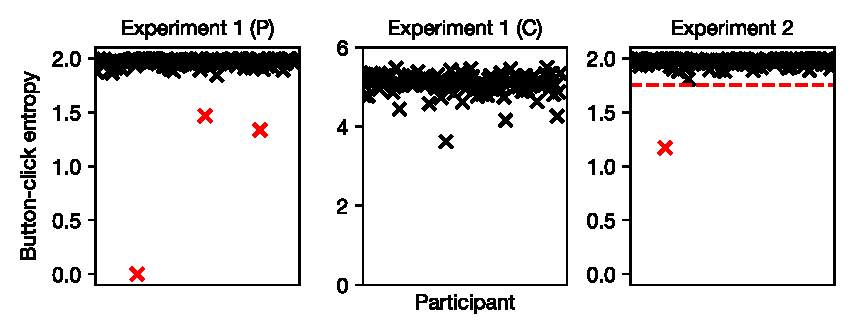
\includegraphics[]{exclusion.eps}
	\caption{Button-click entropy of participants in Experiment~1 (Production and Comprehension) and Experiment~2. Each cross is an individual participant. A total of four participants were excluded, highlighted in red.}
	\label{fg_exclusion}
	\end{center}
	\end{figure}

Under the Production test type of Experiment~1, there were three clear outliers (highlighted in red), so these participants were excluded and new participants were recruited to take their place (all three had been assigned to the Size-only category system). Under the Comprehension test type, we might expect to find a little less randomness in button clicks; participants might hover their cursor around one particular area of the stimulus picker and click the closest stimulus that belongs to the target category, resulting in some buttons being used more frequently than others. Since the results indicated no strong outliers, we retained all participants. In Experiment 2, which is production-based, we preset the exclusion criterion to 1.75~bits (shown by the dashed red line in Fig.~\ref{fg_exclusion}), which was set based on the Production results of Experiment~1. Any participant whose button-click entropy was below this value was excluded automatically and a new participant was automatically recruited to fill that generation in the chain. This was applied in just one instance (highlighted in red).

Therefore, a total of four participants (0.85\%) were excluded across the two Experiments. Three from the Production/Size-only condition and one from the iterated learning experiment.

\section{Participant attrition}

It has been shown that online experiments may be adversely affected by high participant attrition (i.e., termination of the experiment before it is completed), especially where attrition may be linked to experimental condition \citep{Zhou:2016}. In our experiments, for example, participants may be more likely to terminate the experiment if they are assigned to a condition where the system is harder to learn. 

A total of 309 participants began Experiment~1. Of these, 66 terminated the experiment prior to completing it, so their data were erased because they were deemed to have withdrawn consent. Participant numbers by condition are presented in Table~\ref{tb_exp1_participant_numbers}. Participants who terminated the experiment were disproportionately likely to have been assigned to the Size-only system or the Comprehension test type. This means that our results may, for~example, overestimate how easy the Size-only system was to learn, under the assumption that participants are more likely to terminate a task if they find it difficult. However, we can only speculate on reasons why participants might have terminated the experiment. A total of 273 participants began Experiment~2. Of these, 48 participants terminated the experiment prior to completing it.

	\begin{table}
	\begin{center}
	\caption{Participant numbers by condition in Experiment 1 (recruited – terminated – excluded)}
	\sffamily
	\small
	\begin{tabular}{llll}
	\hline
	& \bfseries Production & \bfseries Comprehension & \bfseries TOTAL \\ \hline
	\bfseries Angle-only    & 44 – 4 – 0 = 40    & 46 – 6 – 0 = 40    & 90 – 10 – 0 = 80 \\
	\bfseries Size–only     & 50 – 7 – 3 = 40    & 70 – 30 – 0 = 40   & 120 – 37 – 3 = 80 \\
	\bfseries Angle \& Size & 41 – 1 – 0 = 40    & 58 – 18 – 0 = 40   & 99 – 19 – 0 = 80 \\
	\bfseries TOTAL         & 135 – 12 – 3 = 120 & 174 – 54 – 0 = 120 & 309 – 66 – 3 = 240 \\ \hline
	\end{tabular}
	\label{tb_exp1_participant_numbers}
	\end{center}
	\end{table}

%%%%%%%%%%%%%%%%%%%%%%%%%%%%%%%%%%%%%%%%%%%%%%%%%%%%%%%%%%%%%%%%%%%%%%%%%%%%%%%%%%%%%%%%%%%%
\bibliographystyle{apacite}
\bibliography{/Users/jon/master.bib}
%%%%%%%%%%%%%%%%%%%%%%%%%%%%%%%%%%%%%%%%%%%%%%%%%%%%%%%%%%%%%%%%%%%%%%%%%%%%%%%%%%%%%%%%%%%%

\end{document}